\section{Current Work}
\label{sec:current-work}

Our main objective in applying CI-nets to preference reasoning within goal models is to make set-based qualitative conditional preferences more easily usable for requirements modeling, analysis, and negotiation. We are currently pursuing two primary research directions to accomplish this objective. On one hand, we are developing ways to improve the scalability of preference analysis by developing more efficient algorithms for identifying conflicting preferences within CI-nets and for finding the most preferred sets of items as indicated by a CI-net. On the other hand, we are developing tools and related algorithms to support human users in comprehending, refining, and applying the large amount of information embedded in both CI-nets and goal models. Such tool support is especially important to make the analysis of set-based qualitative preferences practical for industrial-scale systems, because such preferences are not easily reduced to quickly understood (but possibly misunderstood) metrics and because requirements negotiation for a large system can be complex and time-consuming.

\subsection{Efficient Conflict Identification}
\label{sec:conflict-id}

Before attempting to draw conclusions from a set of preferences, it is necessary that the preferences be \emph{consistent} with each other, meaning that no preference contradicts any other preference in the set. If conflicting preferences exist, preference reasoning algorithms cannot make any guarantees about the correctness of their results. More importantly, identifying conflicts among stakeholders' expressed preferences early in the requirements engineering process can guide stakeholders toward making important decisions about the purposes and design of the system before large amounts of resources are put into implementing the ``wrong'' system. 

\begin{figure}%
\centering
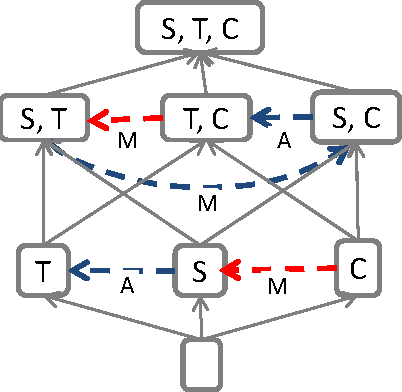
\includegraphics[width=0.5\columnwidth]{./figs/ipg-multi-stakeholder-cropped.pdf}%
\caption{Induced preference graph for CI-net with preferences P1, P2, and P3}%
\label{fig:ipg-with-conflict}%
\end{figure}

Revisiting our example from Section~\ref{sec:cinet}, we observe that 
%while the preferences of all stakeholders must be respected,
conflicts arise when stakeholders specify opposing preferences. For
example, suppose that the manager adds another preference P3,
``Security is more important than Traceability'', to the preference set. 
This can be written as the following CI-net statement:
\begin{quote}
\begin{enumerate}
	\item[(P3)] $\{\}, \{\} : \{S\}, \{C\}$
\end{enumerate}
\end{quote}
Figure~\ref{fig:ipg-with-conflict} shows the IPG for this new set of preferences, with the additional 
edges/flips induced by P3 shown in red. Note that the
new IPG has cycles, indicating that the combined preferences are no longer consistent. 
One can reason that among the sets of NFPs, $(S,C)$ is preferred to $(S,T)$
due to P1, which is in turn preferred to $(T,C)$ due to P3, which is in turn preferred
to $(S,C)$ due to P2. How can such conflicts be detected and resolved?


The preferences specified in a given CI-net are consistent if and only if the IPG for the CI-net is acyclic~\cite{Bouveret:IJCAI2009}. In~\cite{Santhanam:AAAI2010}, we used model checking to perform path-based reachability analysis on IPGs; under this approach, a given CI-net is consistent if and only if all paths through the CI-net's IPG that start at the ``bottom'' of the IPG (where no preference items are provided) eventually reach the ``top'' of the IPG (where all preference variables are provided). The results of this model checking-based algorithm have been proven correct in~\cite{Santhanam:AAAI2010} and are simple to implement using existing model checking tools. Unfortunately, this algorithm does not scale well to large CI-nets (e.g., those with more than 10 total preference items), as $\Theta(2^N)$ time is required to construct the explicit IPG before the reachability analysis can begin. Another approach for verifying consistency among preferences would be to use an optimal algorithm for finding strongly-connected components in a graph, such as Tarjan's algorithm~\cite{Tarjan:DFS}. In this case, absence of strongly-connected components indicates a consistent set of preferences. However, although Tarjan's algorithm runs in linear time, $\Theta(2^N)$ time is still needed to construct the IPG to be searched for strongly connected components.

To improve the scalability of consistency checking for CI-nets, we are exploring a ``syntactic'' approach to consistency checking that will correctly report any conflicts between preferences without explicitly constructing the full IPG. This approach is based on our observation that certain patterns within CI-net statements give rise to cycles in the corresponding IPG. For example, the CI-net statement 
\begin{quote}
\{\}, \{\} : \{\emph{Low Operating Cost}\} \\
$\pref$ \{\emph{Low Operating Cost, High Throughput}\}
\end{quote}
contradicts the monotonicity preference in a CI-net, which implies that \{\emph{Low Operating Cost, High Throughput}\} is preferred to \{\emph{Low Operating Cost}\}. 
%In this case, stakeholders would need to decide which preference is correct and update the preference model accordingly. 
Given CI-net statements of the form shown in Section~\ref{sec:cinet}, conflicts of this type can be found by simply examining each CI-net statement to see whether the \emph{less-preferred-items} set includes every item in the \emph{more-preferred-items} set; examining the entire IPG is not necessary. We are working to identify more complex patterns within either individual CI-net statements or sets of statements that, if present, would indicate either the presence or absence of cycles in the corresponding induced preference graph. Ideally, this will allow us to identify all conflicts between specific preference statements in a given CI-net without incurring the substantial overhead needed to construct the induced preference graph. Even if this is not possible, we anticipate that we will be able to use limited syntactic analysis of CI-net preferences to improve the scalability of consistency checking by (a) identifying classes of CI-nets whose preferences can be efficiently verified as consistent or inconsistent and (b) identifying the parts of an IPG that must be constructed and analyzed to decide consistency, thus eliminating the need to construct the full IPG.
%(\textbf{TODO summarize work that will go into ADT paper on syntactic consistency checking})

Scalable techniques for consistency checking are clearly needed to enable automated reasoning over large, complex sets of preferences. However, our vision for this aspect of our work goes beyond this immediate objective. We believe that scalable CI-net consistency checking can and should be used to improve system stakeholders' awareness of conflicts and tradeoffs among competing preferences for the system. If stakeholders are aware of these conflicts and tradeoffs, which are often not apparent until the first prototypes of the system are built, they can find mutually acceptable solutions to these problems earlier in the system development cycle, saving significant amounts of time, money, and stress.

%(\textbf{TODO write this section as prose.}) Expected outline:
%\begin{enumerate}
	%\item Why it's important: Cannot reason with a set of conflicting (circular) preferences. Conflicts between preferences must be resolved before identifying most preferred alternative(s), in order to guarantee correct results.
	%\item Past work: Model-checking approach to consistency checking (\textbf{TODO summarize from past papers}): correct and easy to implement, but requires explicit IPG. Could use Tarjan's SCC detection algorithm, but still requires time and space costs to construct the entire IPG ($\Theta(2^N)$, where $N$ is the number of variables).
	%\item Current work: (\textbf{TODO summarize work that will go into ADT paper on syntactic consistency checking})
	%\item Future vision: Guiding stakeholders to (a) be aware of conflicts between preferences and (b) find mutually acceptable solutions to such conflicts.
%\end{enumerate}
%

\subsection{Efficient Identification of Preferred Alternatives}
\label{sec:pref-alt}

Once conflicts are identified and removed from the set of preferences, it becomes possible to identify the most preferred sets of properties that the system could have. Knowing this information allows stakeholders to identify possible implementations of the desired system that provide the most preferred sets of properties. If no such implementation exists, it should be possible for stakeholders to obtain an approximately equally preferred or next-most-preferred set of system properties. Ideally, reasoning over qualitative preferences for various properties of the system would go hand-in-hand with analysis of the possible configurations or implementation of the system specified in a goal model within the GORE methodology. As with consistency checking, though, this family of problems is computationally difficult.

The problem of deciding whether one set of items is preferred to another is known as \emph{dominance testing}. Although the dominance testing problem is PSPACE-complete in the general case~\cite{Bouveret:IJCAI2009}, we have presented in~\cite{Oster:FACS12} a model checking-based approach for CI-net dominance testing that identifies the most-preferred set of system properties (CI-net variables) in a reasonable amount of time and space (less than one second and 7 MB of memory) for relatively small CI-nets (up to 16 statements and 10 variables) on a standard Windows laptop. Using this approach, the costs of finding the second-most preferred, third-most preferred, etc.~sets of properties are about the same as the cost of finding the most preferred set of properties. The approach is based on modeling the IPG for a CI-net as a Kripke structure, using model checking to verify the Kripke structure against specially formed temporal-logic properties, and gradually constructing a weak total order over all possible combinations of system properties (CI-net preference items). The weak total order produced by this analysis is consistent with the partial order induced over sets of system properties by the IPG. In~\cite{Oster:ASE11}, we illustrated how this preference reasoning framework can be connected to analysis of goal models in the GORE methodology to identify promising implementations of a desired system.

As with checking the consistency of a set of preferences, scalability is still a major challenge when it comes to identifying highly preferred sets of system properties and for identifying feasible implementations of a proposed system that best satisfy the preferences of the system's stakeholders. Our group's current work in this area involves exploring several possible avenues for more efficient identification of preferred alternatives. One possible approach involves representing preferences using alternative formalisms, such as binary decision diagrams (BDDs), which have been used in efficient algorithms for solving related problems in model checking. Since possible implementations of a system can be identified as satisfiable assignments to a goal models~\cite{Mylopoulos:CAiSE04}, we are also interested in seeing how the latest advances in algorithms and tools like satisfiability (SAT) and satisfiability modulo theorem (SMT) solvers might be applied to prioritize possible system implementations in descending order of preference, as well as the role that tools from the Knowledge Representation and Reasoning community as described in~\cite{Borgida:AIRE14} may be able to play. Additionally, our group is working to identify heuristics for finding approximately optimal system implementations much more efficiently than exhaustive methods might allow. The objective of this research direction is to discover creative algorithmic solutions to analyze CI-nets and their corresponding goal models in a reasonable amount of time and space, even for industry-scale systems and their large, complex requirement and preference models. 

%(\textbf{TODO write this section as prose.}) Expected outline:
%\begin{enumerate}
	%\item Why it's important: (\textbf{TODO make scalability argument})
	%\item Past work: Existing iPref-R framework~\cite{?}, which uses model checking over Kripke structure encoding of IPG to identify next-most-preferred alternative (\textbf{TODO summarize from previous papers}).
	%\item Current work: Exploring alternative representations of preferences (e.g., BDDs), advanced algorithms and tools for analyzing goal model/CI-net combination (e.g., SAT/SMT-solving), heuristics for faster processing with approximately optimal results, etc.
	%\item Future vision: Analyzing CI-nets and their corresponding goal models in a reasonable amount of time and space, even for industry-scale systems. This will require creative algorithmic solutions to avoid the exponential blowup inherent in the general case.
%\end{enumerate}



\subsection{Improved Comprehension of Preference Information}
\label{sec:pref-usability}

One of the core problems in requirements engineering is ensuring traceability between requirements and the information from which those requirements were derived. In the words of Pinheiro and Goguen in~\cite{Pinheiro:IEEESoftware96}, ``Requirements traceability refers to the ability to define, capture and follow the traces left by requirements on other elements of the software development environment and the trace left by those elements on requirements.'' Clearly, many system requirements are affected by the preferences of the system's stakeholders, so it is important to provide traceability between preferences and their corresponding requirements.
However, a requirements engineering process for even a relatively small, simple system can produce a large amount of information, and this problem is only heightened by the addition of detailed preference information to the process. Even with formalisms such as goal models and CI-nets that provide a basic organizational structure for this information, there may be too much information for a requirements specialist, much less an ordinary system stakeholder, to process at a glance. 

Our past work in this area includes the iPref-R framework, which provides tool support to assist end users with preference analysis using CI-nets. iPref-R, which is available at \url{http://fmg.cs.iastate.edu/project-pages/GUI-iPref-R/}, currently provides a graphical front-end for analysis of CI-net and [T]CP-net preferences using our model checking-based approaches. The iPref-R front-end guides users through the process of creating a CI-net while hiding the complexity of the underlying preference language, then assists users in checking their specified preferences for consistency and identifying the most preferred combinations of properties. Although the current GUI for iPref-R is helpful, it falls short of the ideal in that it does not allow users to visualize the space of possible system designs or interactively explore conflicts between preferences.

One of the long-term goals of our research in this area is the development of tools and techniques for visualizing preference and requirement data in ways that allow stakeholders to see interactively what tradeoffs exist; which stakeholders expressed which preferences; or how various requirements, properties, and preferences depend on one another. Our current work in this area involves developing an easily understood visualization of the IPG induced by a given CI-net. This visualization will display basic information about preferences among possible system properties, but users will also be able to interactively query the visualization to find out more detailed information that traces preferences to specific stakeholders or to items in the set of system requirements. Users of this visualization will also be able to discover the tradeoffs that are represented in the goal model and the preference model, which will allow them to explore how these tradeoffs affect the space of possible system design choices.

Our eventual vision for this research direction is to produce a well-designed, easy-to-use ``requirement model dashboard'' that allows requirements engineers and stakeholders alike to comprehend the evolving requirement base, along with the constraints, preferences, and tradeoffs that influenced the choice of requirements used to implement the system, each traceable to a specific source.

%(\textbf{TODO write this section as prose.}) Expected outline:
%\begin{enumerate}
	%\item Why it's important: Too much information for requirements engineers and (especially) system stakeholders to process. In a large body of requirements information, nobody really has any idea what tradeoffs exist; which stakeholders expressed which preferences; or how various requirements, properties, and preferences depend on one another.
	%\item Past work: iPref-R tool support for CI-net/TCP-net preference analysis. iPref-R currently provides a front-end for analysis of CI-net and [T]CP-net preferences using our model checking-based approaches. (\textbf{TODO insert material from ICSE'13 tool paper submission?}) Current GUI is helpful in that it guides users through the process of specifying CI-net statements, but falls short in the area of visualizing the ``space'' of possible system designs or finding conflicts between preferences.
	%\item Current work: Visualizing IPG induced by a CI-net, producing an interactive model that can be queried (e.g, which preferences (as CI-net statements) are in direct conflict, which stakeholder expressed a given preference, which sets of NFRs/softgoals/optional goals can actually be). (\textbf{TODO summarize Zach's students' progress on a tool for CI-net preference and conflict visualization})
	%\item Future vision: A well-designed, easy-to-use ``requirement model dashboard'' that allows requirements engineers and stakeholders alike to comprehend the evolving requirement base, along with the constraints, preferences, and tradeoffs that influenced the choice of requirements used to implement the system, each traceable to a specific source.
%\end{enumerate}
